%%%%%%%%%%%%%%%%%%%%%%%%%%%%%%%%%%%%%%%%%
% Lachaise Assignment
% LaTeX Template
% Version 1.0 (26/6/2018)
%
% This template originates from:
% http://www.LaTeXTemplates.com
%
% Authors:
% Marion Lachaise & François Févotte
% Vel (vel@LaTeXTemplates.com)
%
% License:
% CC BY-NC-SA 3.0 (http://creativecommons.org/licenses/by-nc-sa/3.0/)
%
%%%%%%%%%%%%%%%%%%%%%%%%%%%%%%%%%%%%%%%%%

%----------------------------------------------------------------------------------------
%	PACKAGES AND OTHER DOCUMENT CONFIGURATIONS
%----------------------------------------------------------------------------------------

\documentclass{article}
\usepackage{hyperref}

\newcommand{\hint}{\textbf{Hint:}}


%%%%%%%%%%%%%%%%%%%%%%%%%%%%%%%%%%%%%%%%%
% Lachaise Assignment
% Structure Specification File
% Version 1.0 (26/6/2018)
%
% This template originates from:
% http://www.LaTeXTemplates.com
%
% Authors:
% Marion Lachaise & François Févotte
% Vel (vel@LaTeXTemplates.com)
%
% License:
% CC BY-NC-SA 3.0 (http://creativecommons.org/licenses/by-nc-sa/3.0/)
% 
%%%%%%%%%%%%%%%%%%%%%%%%%%%%%%%%%%%%%%%%%

%----------------------------------------------------------------------------------------
%	PACKAGES AND OTHER DOCUMENT CONFIGURATIONS
%----------------------------------------------------------------------------------------

\usepackage{amsmath,amsfonts,stmaryrd,amssymb} % Math packages

\usepackage{enumerate} % Custom item numbers for enumerations

\usepackage[ruled]{algorithm2e} % Algorithms

\usepackage[framemethod=tikz]{mdframed} % Allows defining custom boxed/framed environments

\usepackage{listings} % File listings, with syntax highlighting
\lstset{
	basicstyle=\ttfamily, % Typeset listings in monospace font
}

%----------------------------------------------------------------------------------------
%	DOCUMENT MARGINS
%----------------------------------------------------------------------------------------

\usepackage{geometry} % Required for adjusting page dimensions and margins

\geometry{
	paper=a4paper, % Paper size, change to letterpaper for US letter size
	top=2.5cm, % Top margin
	bottom=3cm, % Bottom margin
	left=2.5cm, % Left margin
	right=2.5cm, % Right margin
	headheight=14pt, % Header height
	footskip=1.5cm, % Space from the bottom margin to the baseline of the footer
	headsep=1.2cm, % Space from the top margin to the baseline of the header
	%showframe, % Uncomment to show how the type block is set on the page
}

%----------------------------------------------------------------------------------------
%	FONTS
%----------------------------------------------------------------------------------------

\usepackage[utf8]{inputenc} % Required for inputting international characters
\usepackage[T1]{fontenc} % Output font encoding for international characters

\usepackage{XCharter} % Use the XCharter fonts

%----------------------------------------------------------------------------------------
%	COMMAND LINE ENVIRONMENT
%----------------------------------------------------------------------------------------

% Usage:
% \begin{commandline}
%	\begin{verbatim}
%		$ ls
%		
%		Applications	Desktop	...
%	\end{verbatim}
% \end{commandline}

\mdfdefinestyle{commandline}{
	leftmargin=10pt,
	rightmargin=10pt,
	innerleftmargin=15pt,
	middlelinecolor=black!50!white,
	middlelinewidth=2pt,
	frametitlerule=false,
	backgroundcolor=black!5!white,
	frametitle={Command Line},
	frametitlefont={\normalfont\sffamily\color{white}\hspace{-1em}},
	frametitlebackgroundcolor=black!50!white,
	nobreak,
}

% Define a custom environment for command-line snapshots
\newenvironment{commandline}{
	\medskip
	\begin{mdframed}[style=commandline]
}{
	\end{mdframed}
	\medskip
}

%----------------------------------------------------------------------------------------
%	FILE CONTENTS ENVIRONMENT
%----------------------------------------------------------------------------------------

% Usage:
% \begin{file}[optional filename, defaults to "File"]
%	File contents, for example, with a listings environment
% \end{file}

\mdfdefinestyle{file}{
	innertopmargin=1.6\baselineskip,
	innerbottommargin=0.8\baselineskip,
	topline=false, bottomline=false,
	leftline=false, rightline=false,
	leftmargin=2cm,
	rightmargin=2cm,
	singleextra={%
		\draw[fill=black!10!white](P)++(0,-1.2em)rectangle(P-|O);
		\node[anchor=north west]
		at(P-|O){\ttfamily\mdfilename};
		%
		\def\l{3em}
		\draw(O-|P)++(-\l,0)--++(\l,\l)--(P)--(P-|O)--(O)--cycle;
		\draw(O-|P)++(-\l,0)--++(0,\l)--++(\l,0);
	},
	nobreak,
}

% Define a custom environment for file contents
\newenvironment{file}[1][File]{ % Set the default filename to "File"
	\medskip
	\newcommand{\mdfilename}{#1}
	\begin{mdframed}[style=file]
}{
	\end{mdframed}
	\medskip
}

%----------------------------------------------------------------------------------------
%	NUMBERED QUESTIONS ENVIRONMENT
%----------------------------------------------------------------------------------------

% Usage:
% \begin{question}[optional title]
%	Question contents
% \end{question}

\mdfdefinestyle{question}{
	innertopmargin=1.2\baselineskip,
	innerbottommargin=0.8\baselineskip,
	roundcorner=5pt,
	nobreak,
	singleextra={%
		\draw(P-|O)node[xshift=1em,anchor=west,fill=white,draw,rounded corners=5pt]{%
		Question \theQuestion\questionTitle};
	},
}

\newcounter{Question} % Stores the current question number that gets iterated with each new question

% Define a custom environment for numbered questions
\newenvironment{question}[1][\unskip]{
	\bigskip
	\stepcounter{Question}
	\newcommand{\questionTitle}{~#1}
	\begin{mdframed}[style=question]
}{
	\end{mdframed}
	\medskip
}

%----------------------------------------------------------------------------------------
%	WARNING TEXT ENVIRONMENT
%----------------------------------------------------------------------------------------

% Usage:
% \begin{warn}[optional title, defaults to "Warning:"]
%	Contents
% \end{warn}

\mdfdefinestyle{warning}{
	topline=false, bottomline=false,
	leftline=false, rightline=false,
	nobreak,
	singleextra={%
		\draw(P-|O)++(-0.5em,0)node(tmp1){};
		\draw(P-|O)++(0.5em,0)node(tmp2){};
		\fill[black,rotate around={45:(P-|O)}](tmp1)rectangle(tmp2);
		\node at(P-|O){\color{white}\scriptsize\bf !};
		\draw[very thick](P-|O)++(0,-1em)--(O);%--(O-|P);
	}
}

% Define a custom environment for warning text
\newenvironment{warn}[1][Warning:]{ % Set the default warning to "Warning:"
	\medskip
	\begin{mdframed}[style=warning]
		\noindent{\textbf{#1}}
}{
	\end{mdframed}
}

%----------------------------------------------------------------------------------------
%	INFORMATION ENVIRONMENT
%----------------------------------------------------------------------------------------

% Usage:
% \begin{info}[optional title, defaults to "Info:"]
% 	contents
% 	\end{info}

\mdfdefinestyle{info}{%
	topline=false, bottomline=false,
	leftline=false, rightline=false,
	nobreak,
	singleextra={%
		\fill[black](P-|O)circle[radius=0.4em];
		\node at(P-|O){\color{white}\scriptsize\bf i};
		\draw[very thick](P-|O)++(0,-0.8em)--(O);%--(O-|P);
	}
}

% Define a custom environment for information
\newenvironment{info}[1][Info:]{ % Set the default title to "Info:"
	\medskip
	\begin{mdframed}[style=info]
		\noindent{\textbf{#1}}
}{
	\end{mdframed}
}
 % Include the file specifying the document structure and custom commands

%----------------------------------------------------------------------------------------
%	ASSIGNMENT INFORMATION
%----------------------------------------------------------------------------------------

\title{MPhys Lab: Exploring the Hubble Ultra Deep Field} % Title of the assignment

\author{Stephen Wilkins\\ \texttt{s.wilkins@sussex.ac.uk}} % Author name and email address

\date{University of Sussex --- \today} % University, school and/or department name(s) and a date

%----------------------------------------------------------------------------------------

\begin{document}

\maketitle % Print the title

%----------------------------------------------------------------------------------------
%	INTRODUCTION
%----------------------------------------------------------------------------------------

\section*{Introduction} % Unnumbered section

The Hubble Ultra Deep Field (HUDF), also known (due to a re-branding exercise) as the eXtreme Deep Field (XDF), is the {\em Hubble Space Telescope}'s deepest view of the Universe\footnote{\url{http://xdf.ucolick.org}}. The HUDF

The aim of this project is to become familiar with analysing Hubble imaging using \texttt{python}. The ultimately goal is to identify candidate high-redshift galaxies.


\subsection*{Astronomical images}

Astronomical cameras are typically sensitive to a broad wavelength range. To gain spectral information we must combine the camera (detector) with a filter that is only transparent to light over a (typically) small range of wavelengths, typically $\mathcal{O}(100nm)$. These individual images are monochromatic (i.e. they contain no colour information) and can thus be represented by a simple two-dimensional array where each element of the array denotes the signal in that pixel. Images in several filters, or bands, can be combined, as we'll see to generate colour images.

Astronomical images are typically held in the \href{https://en.wikipedia.org/wiki/FITS}{Flexible Image Transport System (FITS)}. In addition to the raw image data FITS file can also contain meta-data in a header and even tabular data. Examples of this meta-data are the values necessary to convert from pixel coordinates (e.g. $(x,y)$) to a position on the sky.

\subsubsection*{Uncertainties}

Having quantified uncertainties (errors) is a critical ingredient in science. There are actually several different ways to estimate the uncertainty on, for example, the flux of an object. However, the best is when a noise (often expressed as a weight) image is provided.

\subsection*{About the HUDF images}

Hubble imaging of the HUDF consists of imaging in 8 optical and near-IR filters stretching from the blue end of the optical (~400nm) to almost 2000nm in the near-IR. These filters are named (from blue to red) f435w, f606w, f775w, f850lp, f105w, f125w, f140w, and f160w. The first 4 were obtained with the Advanced Camera for Surveys (ACS) while the final 4 were obtained with Wide Field Camera 3 (WFC3). The filter transmission curves for these filters, showing the fraction of light transmitted through each filter as a function of wavelength, are shown in Figure \ref{fig:filters}.

For each filter there are a pair of images: a science (sci) and weight (wht) image. These respectively contain the signal in electrons per second (e/s), and an estimate of the noise in each pixel. The noise can be estimated from the weight according to:
\[
{\rm noise} = \frac{1}{\sqrt{\rm weight}}
\]

Because of the way these high-level science images were constructed most of the pixels in these images are actually empty (unobserved). For this reason a mask is also provided allowing you to easily mask empty and other unwanted pixels.

\begin{figure}\label{fig:filters}
	\centering
	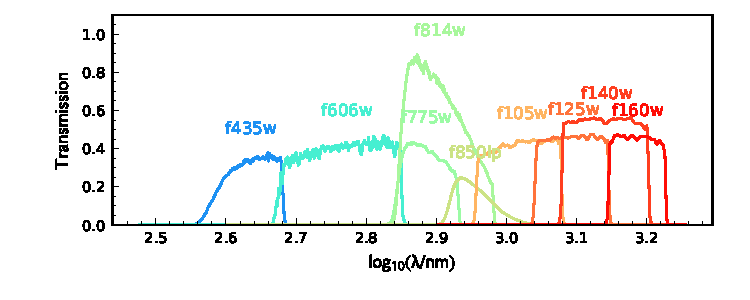
\includegraphics[width=0.8\textwidth]{../utility/filters.pdf}
	\caption{Hubble filters used to observe the HUDF.}
\end{figure}


\subsection*{This project}

In this project you will learn how to analyse {\em Hubble} images using \texttt{python} through a series of task. In addition to \texttt{numpy}, \texttt{scipy}, and \texttt{matplotlib}, you will also need to install \href{https://www.astropy.org}{\texttt{astropy}} and \href{https://photutils.readthedocs.io/en/stable/}{\texttt{photuils}}. To aid you there are a series of examples in \texttt{examples/}.

\section{Basic image analysis} % Numbered section

We'll begin with a few basic \texttt{python} image analysis tasks to get you started.

\subsection{Working with pixels}

First, we'll look at analysing the pixel data in the image. \texttt{example1.py} demonstrates how to read in the image data and convert it to an array of pixel values.

% Numbered question, with an optional title
\begin{question}[\itshape Pixel distribution]
First, model the noise as a gaussian centred at zero and estimate $\sigma$ for the F105W band. \hint\ there should be no signal contribution to the negative pixels so you can use them to measure $\sigma$. To do this first exclude positive pixels. $\sigma$ will then simply be $-P_{31.7}$ (i.e. the negative of the 31.7th percentile). Next, exclude pixels with magnitude $>10\sigma$ and plot both a density histogram (\hint\ use \texttt{plt.hist(..., density = True)}) of the pixel distribution and a normal distribution with the same $\sigma$ as you've just calculated. They won't align perfectly as the pixel distribution unsurprisingly contains more positive pixels.
\end{question}


\subsection{Making plots of images}

We'll now look at exploring some image data. The image data you've read in is simply stored as a 2D array of pixel values. As such we can simply use \texttt{plt.imshow(image)} to produce a plot of the image. \texttt{example2.py} demonstrates how to do this.

\begin{question}[\itshape (with optional title)]
Produce plots of each un-masked weight map. You should do this efficiently with a loop: \textbf{do not} simply repeat the code 8 times. You should notice that the weight maps for the f435w, f606w, f775w, and f850lp are different from those for f105w, f125w, f140w, and f160w. This is because images in the former filters were obtained using the advanced camera for surveys (ACS) instrument while the latter were obtained with Wide Field Camera 3 (WFC3). ACS and WFC3 have different field-of-views. For the WFC3 filters also notice the "holes" in the weight maps corresponding to bad areas of the detector (camera).
\end{question}



\subsection{Combining (stacking) images}

A common task is to combine images either taken with the same filter (often) or with different filters (occasionally). Doing so boosts the sensitivity of the image, albeit, in the latter case, at the expense of the loss of spectral information. To optimise the sensitivity images should be combined by weighting each image with its corresponding weight image. An example of this process is shown in \texttt{example4.py}.


\subsection{Making colour images}

Most people's experience with {\em Hubble} imaging is from the glorious colour images available \href{https://hubblesite.org}{here}. As explained in the introduction {\em Hubble}'s does not capture 'colour' iamges. Instead images in multiple filters are combined together. To obtain 'full-colour' requires at least 3 filters, thereby mimicing the human visual system. The simplest application is to simply map 3 filters to the red (R), green (G), and blue (B) channels. \texttt{example3.py} demonstrates how to do this using 3 of the ACS bands.

\begin{question}[\itshape (with optional title)]
Using  \texttt{example3.py} and \texttt{example4.py} as guides produce a false-colour image of the entire masked XDF using \underline{all 8 filters}. You should define 3 groups of consecutive filters (e.g. \texttt{['f435w','f606w'], ['f775w','f850lp'], ['f105w','f125w','f140w','f160w']}), combine each group, and then combine those stacks together into an RGB image. Congratulations you've now created your own pretty HUDF image. By choosing different filters in each group and playing with the scaling you can make an entirely unique and original version.
\end{question}






%----------------------------------------------------------------------------------------
%	PROBLEM 2
%----------------------------------------------------------------------------------------



\setcounter{Question}{0}
\section{Detecting and measuring sources}

Proin lobortis efficitur dictum. Pellentesque vitae pharetra eros, quis dignissim magna. Sed tellus leo, semper non vestibulum vel, tincidunt eu mi. Aenean pretium ut velit sed facilisis. Ut placerat urna facilisis dolor suscipit vehicula. Ut ut auctor nunc. Nulla non massa eros. Proin rhoncus arcu odio, eu lobortis metus sollicitudin eu. Duis maximus ex dui, id bibendum diam dignissim id. Aliquam quis lorem lorem. Phasellus sagittis aliquet dolor, vulputate cursus dolor convallis vel. Suspendisse eu tellus feugiat, bibendum lectus quis, fermentum nunc. Nunc euismod condimentum magna nec bibendum. Curabitur elementum nibh eu sem cursus, eu aliquam leo rutrum. Sed bibendum augue sit amet pharetra ullamcorper. Aenean congue sit amet tortor vitae feugiat.


\begin{question}[\itshape (with optional title)]
First of all, following \texttt{example3.py}, create a detection science and weight image by stacking the F105W, F125W, F140W, and F160W images together. You will use this image to detect faint sources.
\end{question}

\subsection{Significance maps}

\begin{question}[\itshape (with optional title)]
Create a significance map of a 400 pixel wide area centred on (3100, 1800).
\end{question}


\subsection{Segmentation}

Segmentation (\url{https://en.wikipedia.org/wiki/Image_segmentation}) is one way of detecting sources (objects) in an image. In the simplest implementation we can identify collections of connected pixels which are all above some threshold. \texttt{example6.py} demonstrates the use of simple segmentation routines using the \texttt{astropy.photutils} module.

\begin{question}[\itshape (with optional title)]
Create a segmentation image (with no de-blending) of the same region you looked at in 2b. Assuming $n_{\rm pixels} = 5$ and ${\rm threshold} = 2.5$. Next, systematically explore the impact of changing $n_{\rm pixels}$ (must be an integer) and ${\rm threshold}$ on the number of sources detected.
\end{question}


\begin{question}[\itshape (with optional title)]
Sticking with $n_{\rm pixels} = 5$ and ${\rm threshold} = 2.5$ now explore the impact of the parameters that control de-blending on the number of sources.
\end{question}


\subsection{Measuring the signal (and noise) of sources}


\begin{question}[\itshape Measure the signal of all sources]
Measure the signal (e/s) of all the sources in the region. To do this you can combine the segmentation map with the detection science image. Plot a histogram. Do the same for the de-blended image and discuss the difference.
\end{question}


\begin{question}[\itshape Make a multi-band catalogue]
Using the original (un-blended) segmentation map measure the signal and noise (or error) of every object in every single filter and create a catalogue using a dictionary. Save this catalogue for use later.
\end{question}



%----------------------------------------------------------------------------------------
%	Part 3
%----------------------------------------------------------------------------------------

\setcounter{Question}{0}
\section{Finding distant galaxies}

High-redshift galaxies can be identified using the Lyman-break technique. This takes advantage of a strong break in the spectrum of galaxies caused by the absorption of ionising photons by inter-stellar and inter-galactic hydrogen.

\subsection{Changing units}

The units of the original images are electrons per second (e/s). However, we want units of flux\footnote{Actually spectral flux density.}, for example in nano-\href{https://en.wikipedia.org/wiki/Jansky}{Jansky} (nJy). The conversion from from e/s to nJy depends on the observatory, instrument, and filter, and thus is unique for each filter: \texttt{example9.py} contains the relevant conversion in the form of a dictionary.

\begin{question}[\itshape Convert to flux]
Read in the catalogue you created in Task 2f and convert the signal into a flux (nJy) using the conversion dictionary in \texttt{example9.py}. Plot $f_{f105w}/f_{125w}$ vs. $f_{f850lp}/f_{105w}$ for all the objects in the catalogue.
\end{question}


\subsection{Finding distant galaxies}


Firstly, we want to guard against objects which are detected a low-S/N, as these are more likely to be contaminants (or not even real sources). To do this we can simply place a constraint on the signal-to-noise (S/N) in a filter where we know any real high-redshift object should be detected. We are somewahat free to choose the band and threshold but $f_{\rm f125w}$ and a S/N$>10$ is a reasonable choice.

Next, we know that high-redshft galaxies have a strong spectral break. If the break falls between two bands A and B we'd expect that $f_{\rm A}/f_{\rm B}$ should be small. Galaxies at $z\sim 7$ have a break between the $f850lp$ and $f105w$ bands. A reasonable choice of ratio upper-limit is $\sim 0.4$.

We also expect the shape of the continuum above the break to be flat, or even negative (i.e. decreasing to longer-wavelength). Using a pair of bands above the break (e.g. $f105w$ and $f125w$) we can then place an additional constraint allowing us to further weed out contamination. A reasonable choice for ratio lower-limit is $\sim 0.75$

Finally, any truely high-redshift object should be undetected in any filter shortward of the break. For $z\sim 7$ objects we wouldn't expect them to be detected in $f435w$, $f606w$, or $f775w$. This can be implemented by enforcing that any candidate object is detected at less than S/N$=2$ in those bands.

In conclusion, our selection criteria can be expressed as follows:

\[
S/N(f_{\rm f125w})>10
\]
\[
f_{\rm f850lp}/f_{\rm f105w}<0.4
\]
\[
f_{\rm f105w}/f_{\rm f125w}>0.75
\]
\[
S/N(f_{\rm f435w})<2\, \land\, S/N(f_{\rm f606w})<2\, \land\, S/N(f_{\rm f775w})<2
\]


\begin{question}[\itshape Identifiy high-redshift galaxy candidates]
Add the above flux-ratio criteria to your plot from 3a (either as lines or a shaded region). Apply the criteria to your catalogue of objects and highlight any objects meeting the criteria on your plot.
\end{question}


\begin{question}[\itshape Detection image thumbnail]
Using \texttt{example7.py} as a guide make detection image thumbnail of your candidate(s), if you have any.
\end{question}

\begin{question}[\itshape More thumbnails]
Following on from 3c also make thumbails in each band (\hint\ use \texttt{subplots} for ease) in addition to an RGB thumbnail.
\end{question}

%----------------------------------------------------------------------------------------

\end{document}
